\documentclass[12pt, onecolumn]{article}

% 引入相关的包
\usepackage{amsmath, listings, fontspec, geometry, graphicx, ctex, color, subfigure, amsfonts, amssymb}
\usepackage{multirow}
\usepackage[table,xcdraw]{xcolor}
\usepackage[ruled]{algorithm2e}
\usepackage[hidelinks]{hyperref}

		\usepackage{graphicx}
		\usepackage[most]{tcolorbox}
\hypersetup{
	colorlinks=true,
	linkcolor=red,
	citecolor=red,
}
\usepackage{booktabs}
\usepackage{multirow}
\usepackage{picins}

% 设定页面的尺寸和比例
\geometry{left = 1.5cm, right = 1.5cm, top = 1.5cm, bottom = 1.5cm}

% 设定两栏之间的间距
\setlength\columnsep{1cm}

% 设定字体,为代码的插入作准备
\newfontfamily\ubuntu{Ubuntu Mono}
\newfontfamily\consolas{Consolas}

% 头部信息
\title{\normf{编程:观测值逐次更新的扩展卡尔曼滤波器}}
\author{\normf 姓名:陈烁龙\;\;\;学号:2023202140019\;\;\;学院:测绘学院}
\date{\normf{\today}}

% 代码块的风格设定
\lstset{
	language=C++,
	basicstyle=\small\ubuntu,
	keywordstyle=\textbf,
	stringstyle=\itshape,
	commentstyle=\itshape,
	numberstyle=\scriptsize\ubuntu,
	showstringspaces=false,
	numbers=left,
	numbersep=8pt,
	tabsize=2,
	frame=single,
	framerule=1pt,
	columns=fullflexible,
	breaklines,
	frame=shadowbox, 
	backgroundcolor=\color[rgb]{0.97,0.97,0.97}
}

% 字体族的定义
% \fangsong \songti \heiti \kaishu
\newcommand\normf{\fangsong}
\newcommand\boldf{\heiti}
\newcommand\keywords[1]{\bfseries{关键词:} \normf #1}

\newcommand\liehat[1]{\left[ #1 \right]_\times}
\newcommand\lievee[1]{\left[ #1 \right]^\vee}
\newcommand\liehatvee[1]{\left[ #1 \right]^\vee_\times}

\newcommand\mlcomment[1]{\iffalse #1 \fi}
%\newcommand\mlcomment[1]{ #1 }

\newcommand\bsm[1]{\boldsymbol{\mathrm{#1}}}
\newcommand\rotation[2]{{\bsm{R}_{#1}^{#2}}}
\newcommand\angvel[2]{{\bsm{\omega}_{#1}^{#2}}}
\newcommand\angacce[2]{{\bsm{\alpha}_{#1}^{#2}}}
\newcommand\translation[2]{{\bsm{p}_{#1}^{#2}}}
\newcommand\translationhat[2]{{\hat{\bsm{p}}_{#1}^{#2}}}
\newcommand\linvel[2]{{\bsm{v}_{#1}^{#2}}}
\newcommand\linacce[2]{{\bsm{a}_{#1}^{#2}}}
\newcommand\gravity[1]{{\bsm{g}^{#1}}}
\newcommand\smallminus{{\text{-}}}
\newcommand\smallplus{{\text{+}}}
\newcommand\coordframe[1]{\underrightarrow{\mathcal{F}}_{#1}}

\newcounter{problemname}
\newenvironment{problem}{\stepcounter{problemname}\par\noindent\normf\textbf{\textcolor[rgb]{1,0,0}{题目\arabic{problemname}.} }}{\leavevmode\\\par}
\newenvironment{solution}{\par\noindent\normf\textbf{解答: }}{\leavevmode\\\par}
\newenvironment{note}{\par\noindent\normf\textbf{题目\arabic{problemname}的注记: }}{\leavevmode\\\par}


\begin{document}
	\begin{titlepage}
	    \centering
	    
\includegraphics[width=0.4\textwidth]{whu_red.png}\par\vspace{1cm}
	    \vspace{4cm}
	    {\huge\kaishu\bfseries MI-Calib\par}
	    \vspace{3cm}
	    {\Large\kaishu 
	    \begin{center}\begin{tabular}{l}
	    姓名:陈烁龙\\
	    学号:\bfseries 2023202140019\\
	    学院:测绘学院
	    \end{tabular}\end{center}
	     \par}
	    
	
	    \vfill
	
	% Bottom of the page
	    {\large\kaishu\bfseries \today\par}
	\end{titlepage}
		% 换页
 		\thispagestyle{empty}
		\clearpage
		
		% 插入目录、图、表并换页
		\pagenumbering{roman}
		\tableofcontents
		\newpage
		\listoffigures
%		\newpage
%		\listoftables
		% 罗马字母形式的页码
		
		\clearpage
		% 从该页开始计数
		\setcounter{page}{1}
		% 阿拉伯数字形式的页码
		\pagenumbering{arabic}
	
	\section{\normf{Dynamics}}
	\normf
	\begin{equation}
	\begin{cases}
	\begin{aligned}
	\bsm{a}(\tau)&=\left(\rotation{b}{b_0}(\tau) \right) ^\top\cdot\left(\linacce{b}{b_0}(\tau)-\gravity{b_0}\right) 
	\\
	\bsm{\omega}(\tau)&=\left(\rotation{b}{b_0}(\tau) \right) ^\top\cdot\angvel{b}{b_0}
	\end{aligned}
	\end{cases}
	\end{equation}
	set the body frame as $\coordframe{b^i}$, the reference frame as $\coordframe{b^r_0}$:
	\begin{equation}
	\begin{cases}
	\begin{aligned}
	\bsm{a}^i(\tau)&=\left(\rotation{b^i}{b^r_0}(\tau) \right) ^\top\cdot\left(\linacce{b^i}{b^r_0}(\tau)-\gravity{b^r_0}\right) 
	\\
	\bsm{\omega}^i(\tau)&=\left(\rotation{b^i}{b^r_0}(\tau) \right) ^\top\cdot\angvel{b^i}{b^r_0}(\tau)
	\end{aligned}
	\end{cases}
	\end{equation}
	where $\bsm{a}_i(\tau)$ and $\bsm{\omega}_i(\tau)$ are the linear acceleration and angular velocity output from the $i$-th IMU at time $\tau$, and
	\begin{equation}
	\begin{gathered}
	\rotation{b^i}{b^r_0}(\tau)=\rotation{b^r}{b^r_0}(\tau)\cdot\rotation{b^i}{b^r}
	\\
	\translation{b^i}{b^r_0}(\tau)=\rotation{b^r}{b^r_0}(\tau)\cdot\translation{b^i}{b^r}+\translation{b^r}{b^r_0}(\tau)
	\end{gathered}
	\end{equation}
	thus
	\begin{equation}
	\begin{gathered}
	\angvel{b^i}{b^r_0}(\tau)=\angvel{b^r}{b^r_0}(\tau)
	\\
	\linvel{b^i}{b^r_0}(\tau)=-\liehat{\rotation{b^r}{b^r_0}(\tau)\cdot\translation{b^i}{b^r}}\cdot\angvel{b^r}{b^r_0}(\tau)+\linvel{b^r}{b^r_0}(\tau)
	\\
	\linacce{b^i}{b^r_0}(\tau)=-\liehat{\rotation{b^r}{b^r_0}(\tau)\cdot\translation{b^i}{b^r}}\cdot\angacce{b^r}{b^r_0}(\tau)
	-\liehat{\angvel{b^r}{b^r_0}(\tau)}\cdot
	\liehat{\rotation{b^r}{b^r_0}(\tau)\cdot\translation{b^i}{b^r}}\cdot\angvel{b^r}{b^r_0}(\tau)+\linacce{b^r}{b^r_0}(\tau)
	\end{gathered}
	\end{equation}
	Based on:
	\begin{equation}
	\bsm{\omega}^i(\tau)=\left(\rotation{b^i}{b^r_0}(\tau) \right) ^\top\cdot\angvel{b^i}{b^r_0}(\tau)=\left(\rotation{b^r}{b^r_0}(\tau)\cdot\rotation{b^i}{b^r} \right) ^\top\cdot\angvel{b^r}{b^r_0}(\tau)
	\end{equation}
	the rotation spline of $\coordframe{b^r}$ and the rotation extrinsics $\rotation{b^i}{b^r}$ could be recovered.
	
	
	\section{\normf{Velocity Integration}}
	we have
	\begin{equation}
	\bsm{a}^r(\tau)=\left(\rotation{b^r}{b^r_0}(\tau) \right) ^\top\cdot\left(\linacce{b^r}{b^r_0}(\tau)-\gravity{b^r_0}\right) 
	\qquad
	\bsm{a}^i(\tau)=\left(\rotation{b^i}{b^r_0}(\tau) \right) ^\top\cdot\left(\linacce{b^i}{b^r_0}(\tau)-\gravity{b^r_0}\right) 
	\end{equation}
	thus
	\begin{equation}
	\rotation{b^r}{b^r_0}(\tau) \cdot\bsm{a}^r(\tau)=\linacce{b^r}{b^r_0}(\tau)-\gravity{b^r_0}
	\qquad
	\rotation{b^i}{b^r_0}(\tau) \cdot\bsm{a}^i(\tau)=\linacce{b^i}{b^r_0}(\tau)-\gravity{b^r_0}
	\end{equation}
	and
	\begin{equation}
	\label{equ:vel_pretegration}
	\int_{\tau_k}^{\tau_{k+1}}\rotation{b^r}{b^r_0}(\tau) \cdot\bsm{a}^r(\tau)\cdot d\tau
	=\linvel{b^r}{b^r_0}(\tau_{k+1})-\linvel{b^r}{b^r_0}(\tau_k)-\gravity{b^r_0}\cdot\left(\tau_{k+1}-\tau_k \right) 
	\end{equation}
	for the left part, we have
	\begin{equation}
	\begin{gathered}
	\rotation{b^r}{b^r_0}(\tau) \cdot\bsm{a}^r(\tau)
		=\linacce{b^r}{b^r_0}(\tau)-
		\left( \linacce{b^i}{b^r_0}(\tau)-\rotation{b^i}{b^r_0}(\tau) \cdot\bsm{a}^i(\tau)\right) 
		=\linacce{b^r}{b^r_0}(\tau)-
		\linacce{b^i}{b^r_0}(\tau)+\rotation{b^i}{b^r_0}(\tau) \cdot\bsm{a}^i(\tau) 
	\\
	\linacce{b^r}{b^r_0}(\tau)-\linacce{b^i}{b^r_0}(\tau)=\liehat{\rotation{b^r}{b^r_0}(\tau)\cdot\translation{b^i}{b^r}}\cdot\angacce{b^r}{b^r_0}(\tau)
	+\liehat{\angvel{b^r}{b^r_0}(\tau)}\cdot
	\liehat{\rotation{b^r}{b^r_0}(\tau)\cdot\translation{b^i}{b^r}}\cdot\angvel{b^r}{b^r_0}(\tau)
	\\
	\linacce{b^r}{b^r_0}(\tau)-\linacce{b^i}{b^r_0}(\tau)
	=-\liehat{\angacce{b^r}{b^r_0}(\tau)}\cdot\rotation{b^r}{b^r_0}(\tau)\cdot\translation{b^i}{b^r}
	-\liehat{\angvel{b^r}{b^r_0}(\tau)}\cdot
	\liehat{\angvel{b^r}{b^r_0}(\tau)}\cdot\rotation{b^r}{b^r_0}(\tau)\cdot\translation{b^i}{b^r}
	\\
	\linacce{b^r}{b^r_0}(\tau)-\linacce{b^i}{b^r_0}(\tau)
		=-\left(\liehat{\angacce{b^r}{b^r_0}(\tau)}+ \liehat{\angvel{b^r}{b^r_0}(\tau)}^2\right) \cdot\rotation{b^r}{b^r_0}(\tau)\cdot\translation{b^i}{b^r}
	\end{gathered}
	\end{equation}
	thus
	\begin{equation}
	\rotation{b^r}{b^r_0}(\tau) \cdot\bsm{a}^r(\tau)
	=\rotation{b^r}{b^r_0}(\tau) \cdot\rotation{b^i}{b^r} \cdot\bsm{a}^i(\tau) -\left(\liehat{\angacce{b^r}{b^r_0}(\tau)}+ \liehat{\angvel{b^r}{b^r_0}(\tau)}^2\right) \cdot\rotation{b^r}{b^r_0}(\tau)\cdot\translation{b^i}{b^r}
	\end{equation}
	with the left part of (\ref{equ:vel_pretegration}), we have:
	\begin{equation}
	\int_{\tau_k}^{\tau_{k+1}}\rotation{b^r}{b^r_0}(\tau) \cdot\rotation{b^i}{b^r} \cdot\bsm{a}^i(\tau) \cdot d\tau-
	\int_{\tau_k}^{\tau_{k+1}}\left(\liehat{\angacce{b^r}{b^r_0}(\tau)}+ \liehat{\angvel{b^r}{b^r_0}(\tau)}^2\right) \cdot\rotation{b^r}{b^r_0}(\tau)\cdot d\tau\cdot\translation{b^i}{b^r}
	=\bsm{b}^i_{k,k+1}-\bsm{A}_{k,k+1}\cdot\translation{b^i}{b^r}
	\end{equation}
	we rewrite (\ref{equ:vel_pretegration}):
	\begin{equation}
	\bsm{b}^i_{k,k+1}-\bsm{A}_{k,k+1}\cdot\translation{b^i}{b^r}=
	\linvel{b^r}{b^r_0}(\tau_{k+1})-\linvel{b^r}{b^r_0}(\tau_k)-\gravity{b^r_0}\cdot\left(\tau_{k+1}-\tau_k \right) 
	\end{equation}
	\begin{equation}
	\begin{bmatrix}
	-\bsm{I}_3&\bsm{I}_3&\bsm{A}_{k,k+1}&-\bsm{I}_3\cdot\left(\tau_{k+1}-\tau_k \right) 
	\end{bmatrix}
	\begin{bmatrix}
	\linvel{b^r}{b^r_0}(\tau_k)
	\\
	\linvel{b^r}{b^r_0}(\tau_{k+1})
	\\
	\translation{b^i}{b^r}
	\\
	\gravity{b^r_0}
	\end{bmatrix}=\bsm{b}^i_{k,k+1}
	\end{equation}
	\begin{equation}
	\bsm{H}_{k,k+1}\cdot\bsm{x}^i_{k,k+1}=\bsm{b}^i_{k,k+1}
	\end{equation}
	\begin{equation}
	\left( \bsm{H}_{k,k+1}^\top\cdot\bsm{H}_{k,k+1}\right) \cdot\bsm{x}^i_{k,k+1}=\bsm{H}_{k,k+1}^\top\cdot\bsm{b}^i_{k,k+1}
	\end{equation}
	marginalize $\linvel{b^r}{b^r_0}(\tau_k)$ and $\linvel{b^r}{b^r_0}(\tau_{k+1})$ when solving.
	
	Given a data sequence from $\mathcal{N}$ IMUs, split it into $\mathcal{M}$ blocks, thus we need to estimate parameters with size of:
	\begin{equation}
	\left( \mathcal{N}-1\right) \times 3+2+\left( \mathcal{M}+1\right) \times 3=
	\left(\mathcal{N}+\mathcal{M} \right)\times 3 +2
	\end{equation}
	we have constraints with size of:
	\begin{equation}
	\mathcal{M}\times 3\times \mathcal{N}
	\end{equation}
	when:
	\begin{equation}
	\mathcal{M}\times 3\times \mathcal{N}\ge \left(\mathcal{N}+\mathcal{M} \right)\times 3 +2
	\end{equation}
	we could recover the extrinsic translations and the gravity vector.
	Assume that we have two IMUs, i.e., $\mathcal{N}=2$, then:
	\begin{equation}
	\mathcal{M}\times 3\times 2\ge \left(2+\mathcal{M} \right)\times 3 +2
	\qquad\Rightarrow\qquad
	\mathcal{M}\ge 3\ge \frac{8}{3}
	\end{equation}
	
	
	\newpage
	\bibliographystyle{IEEEtran}
	\bibliography{reference}
		
	\newpage
	\section*{ACKNOWLEDGMENT}
	\begin{tcolorbox}[colback=white,colframe=white!70!black,title={\bfseries Author Information}]
	\par\noindent
		\parbox[t]{\linewidth}{
	 \noindent\parpic{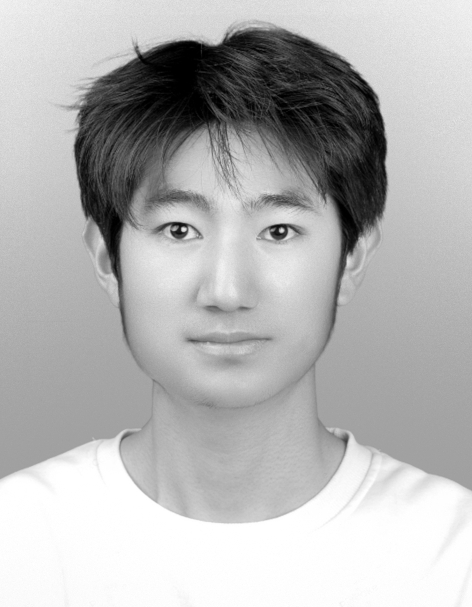
\includegraphics[height=2in,width=1in,clip,keepaspectratio]{ShuolongChen_grey.jpg}}
	 \noindent{\bfseries Shuolong Chen}\emph{
	 received the B.S. degree in geodesy and geomatics engineering from Wuhan University, Wuhan China, in 2023.
	 He is currently a master candidate at the school of Geodesy and Geomatics, Wuhan University. His area of research currently focuses on integrated navigation systems and multi-sensor fusion.
	 Contact him via e-mail: shlchen@whu.edu.cn.
	 }}
	\end{tcolorbox}
		
		
\end{document}
